% === Revtex Declaration ===
\documentclass[aps, 10pt, english, twoside, twocolumn, pra, nofootinbib, tightenlines, longbibliography, superscriptaddress]{revtex4-1}

% === All of the Packages I use frequently ===
\usepackage{document_config}

% === Drafting Declarations ===
\draftprofile[TC Fraser]{TC}{Red}

\begin{document}
    \title{
    A Memory-Efficient Algorithm for Generating Non-Contextuality Inequalities
    }
    \author{Thomas C. Fraser}
    \email{tcfraser@tcfraser.com}
    \affiliation{Perimeter Institute for Theoretical Physics, Waterloo, Ontario, Canada, N2L 2Y5}
    \affiliation{University of Waterloo, Waterloo, Ontario, Canada, N2L 3G1}
    \date{\today}
    \begin{abstract}
        This is the abstract.
    \end{abstract}
    \maketitle
    \tableofcontents

    \section{Introduction}
    \subsection{Applications}

    \section{Marginal Satisfiability}
    \subsection{Definitions}
    To every random variable\footnote{Throughout this document, it is assumed that all random variables are discrete and have finite cardinality.} $v$ there corresponds a prescribed set of \term{outcomes} $\outcomes{v}$ and a set of \term{events over $v$} denoted $\events{v}$ corresponding to the set of all functions of the form $\w : \bc{v} \to \outcomes{v}$. Evidently, $\events{v}$ and $\outcomes{v}$ are isomorphic structures and their distinction can be confounding. There is rarely any harm in referring synonymously to either as outcomes. Nonetheless, a sheaf-theoretic treatment of contextuality \cite{Abramsky_2011} demands the distinction. Specifically for this work, the distinction becomes essential for the exploitation of marginal symmetries in \cref{sec:marginal_symmetries}. As a natural generalization we define the event over a collection of random variables $V = \bc{v_1, \ldots, v_n}$ in a parallel manner:
    \[ \events{V} \defined \bc{\w : V \to \outcomes{V} \mid \forall v \in V, \w\br{v} \in \outcomes{v}} \]
    Furthermore, the \term{domain $\domain{\w}$} of an event $\w$ is the set of random variables it valuates, i.e. if $\w \in \events{V}$ then $\domain{\w} = V$.

    For every $\w \in \events{V}$ and $V' \subset V$, the \term{restriction of $\w$ onto $V'$} (denoted $\restrict{\w}{V'}$) corresponds to the unique event in $\events{V'}$ that agrees with $\w$ for all valuations of variables in $V'$, i.e. $\forall v' \in V': \restrict{\w}{V'}\br{v'} = \w\br{v'}$. Using this notational framework, a probability distribution or simply \term{distribution} $\prob{V}$ is a probability measure on $\events{V}$, assigning to each $\w \in \events{V}$ a real number $\prob{V}\br{\w} \in \bs{0,1}$ such that $\sum_{\w \in \events{V}} \prob{V}\br{\w} = 1$. The set of all distributions over $\events{V}$ is denoted $\probset{V}$. Moreover, given $\prob{V} \in \probset{V}$ and $V' \subset V$, there is an induced distribution $\restrict{\prob{V}}{V'} \in \probset{V'}$ obtained by \textit{marginalizing} $\prob{V}$:
    \[ \restrict{\prob{V}}{V'}\br{\w'} = \sum_{\substack{\w \in \events{V} \\ \restrict{\w}{V'} = \w'}} \prob{V}\br{\w} \eq \label{eq:marginalization_defined} \]
    Presently, the reader is equipped with sufficient notation and terminology to comprehend the marginal problem.
    \begin{definition}
        \term{The Marginal Problem (MP)}: Given a collection of $m$ distributions $\bc{\prob{V_1},\ldots,\prob{V_m}}$, does there exist a distribution $\prob{\jointvar} \in \probset{\jointvar}$ with $\jointvar \defined \bigcup_{i = 1}^{m} V_m$ such that $\forall i : \restrict{\prob{\jointvar}}{V_i} = \prob{V_i}$?
    \end{definition}

    To facilitate further discussion of this problem, several pieces of nomenclature will be introduced. First, the set $\mscenario = \bc{V_1, \ldots, V_m}$ is called the \term{marginal scenario} while its elements are called the \term{marginal contexts}. The collection of distributions $\prob{\mscenariowrap} \defined \bc{\prob{V_1},\ldots,\prob{V_m}}$\footnote{The subscript $*$ preceding $\mscenariowrap$ is added for clarity; $\prob{\mscenariowrap}$ is \textit{not} a distribution but a set of distributions over $\mscenario$. The $\mscenariowrap$ convention is adopted throughout this report.} is called the \term{marginal model}~\cite{Fritz_2011}\footnote{In~\cite{Abramsky_2011}, $\prob{\mscenariowrap}$ is instead called an \textit{empirical model}.}. The distribution $\prob{\jointvar}$, if it exists, is termed the \term{joint distribution}. Strictly speaking, as defined by~\cite{Fritz_2011}, a marginal scenario forms an \textit{abstract simplicial complex}, meaning it satisfies the supplementary requirement that all subsets of contexts are also contexts, i.e. $\forall V \in \mscenario : V' \subset V \implies V' \in \mscenario$. Throughout this work, we exclusively consider (without loss of generality) \textit{maximal} marginal scenarios, restricting our focus to the contexts which are contained in no others. Finally, a marginal model $\prob{\mscenariowrap}$ is said to be \term{non-contextual}, and will be denoted $\prob{\mscenariowrap} \in \noncontextual \subseteq \probset{\mscenariowrap}$ if it admits a joint distribution and \term{contextual} otherwise ($\prob{\mscenariowrap} \in \contextual$). Equipped with this additional terminology and notation, MP now reads: given $\prob{\mscenariowrap}$, is $\prob{\mscenariowrap} \in \noncontextual$ or not?

    \subsection{Linearity}
    An essential feature of MP is linearity; the marginalization of $\prob{\jointvar}$ onto the marginal contexts $\bc{\restrict{\prob{\jointvar}}{V} \mid V \in \mscenario}$ is a linear transformation, requiring only the summations pursuant to \cref{eq:marginalization_defined}. Consequently, it is advantageous to consider the statement of MP as a matrix multiplication. To this end, for each marginal scenario $\mscenario$ we define a binary matrix $\incidence$ called the \term{incidence matrix} which implements this mapping. The columns of $\incidence$ are indexed by \textit{joint events} $j \in \events{\jointvar}$ and the rows are indexed by \textit{marginal events} $m \in \events{V}$ for some $V \in \mscenario$. By deliberate abuse of notation, we will denote the set of all marginal events as $\events{\mscenariowrap}$ and is defined as the following disjoint union:
    \[ \events{\mscenariowrap} \defined \coprod_{V \in \mscenario} \events{V} \]
    The $\abs{\events{\mscenariowrap}}\times\abs{\events{\jointvar}}$ incidence matrix $\incidence$ is then defined element-wise for $m \in \events{\mscenariowrap}$ and $j \in \events{\jointvar}$:
    \[ \incidence^{m}_{j} = \begin{cases}
        1 & \restrict{j}{\domain{m}} = m\\
        0 & \text{otherwise}
    \end{cases} \eq \label{eq:incidence_matrix} \]
    Conceptually, the entries of this matrix are populated with ones whenever the marginal event (row) $m$ is the restriction of some joint event (column) $j$. For a given marginal scenario $\mscenario$, $\incidence$ represents the tuple of restriction maps $\incidence : \events{\jointvar} \to \prod_{V \in \mscenario} \events{V} :: j \mapsto \bc{\restrict{j}{V} \mid V \in \mscenario}$~\cite{Abramsky_2011}. Furthermore, note that the component indices of $\incidence$ in \cref{eq:incidence_matrix} are deliberately separated. Among other reasons, this is done to allow one to denote the $m$-th row of $\incidence$ as $\incidence^{m}$ and the $j$-th column as $\incidence_{j}$. For further notational convenience, since $\incidence$ is a binary matrix, we let $\incidence^{m}$ and $\incidence_{j}$ analogously correspond their respective \textit{supports}\footnote{The \textit{support} $\supp{f}$ of a mapping $f$ is the subset of its domain $\domain{f}$ that is not mapped to a zero element: $\supp{f} = \bc{x \in \domain{f} \mid f\br{x} \neq 0}$.}, e.g. $m \in \supp{\incidence_{j}}$ if and only if $\incidence_{j}^{m} = 1$. Throughout the remainder of this report, the utility of the incidence matrix $\incidence$ will be indispensable.

    To illustrate this concretely, consider the following example. Let $\jointvar$ be $3$ binary variables $\bc{a,b,c}$ and $\mscenario$ be the marginal scenario $\mscenario = \bc{\bc{a,b}, \bc{b,c}, \bc{a,c}}$. The incidence matrix for $\mscenario$ becomes:
    \begin{equation}
        \resizebox{1.0\hsize}{!}{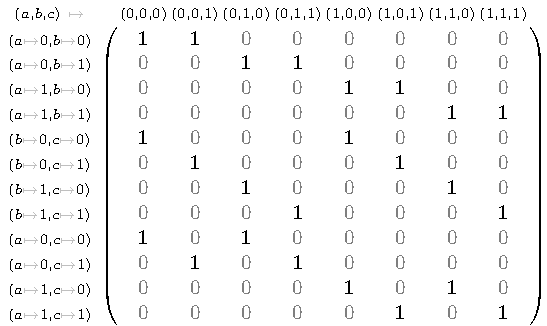
\includegraphics{figures/incidence_matrix_1_example/figure.pdf}}
        \label{eq:incidence_example}
    \end{equation}

    In addition, for any joint distribution $\prob{\jointvar} \in \probset{\jointvar}$ we associate a joint distribution \textit{vector} $\prob{\jointvar}$ (identically denoted) indexed by $j \in \events{\jointvar}$, i.e. $\prob{\jointvar}^{j} \defined \prob{\jointvar}\br{j}$. Analogously, for each marginal model $\prob{\mscenariowrap} \in \probset{\mscenariowrap}$ there is an associated marginal distribution \textit{vector} $\prob{\mscenariowrap}$ indexed by $m \in \events{\mscenariowrap}$ such that $\prob{\mscenariowrap}^{m} \defined \prob{\domain{m}}\br{m}$. Using these vectors, the marginal problem becomes the following linear program:

    \begin{definition}
        \label{def:MLP}
        \term{The Marginal Linear Program (MLP)}:
        \begin{alignat*}{2}
            & \text{minimize:} \quad&& \emptyset \cdot \prob{\jointvar} \footnotemark\\
            & \text{subject to:} && \prob{\jointvar} \succeq 0 \\
            & && \incidence \cdot \prob{\jointvar} = \prob{\mscenariowrap} \eq \label{eq:incidence_marginal_problem}
        \end{alignat*}
    \end{definition}
    \addtocounter{footnote}{-1} % Why do I have to do this? Is it because of the secondary text environment in the alignat?
    \footnotetext{Note that the primal value of the linear program is of no interest, all that matters is its \textit{feasibility}. Here $\emptyset$ denotes a null vector of all zero entries.} As such, $\prob{\mscenariowrap} \in \noncontextual$ if and only if MLP is a \textit{feasible} linear program. Importantly, if MLP is feasible, it will return the joint distribution $\prob{\jointvar}$. To every linear program, there exists a dual linear program that characterizes the feasibility of the original~\cite{Schrijver_1998}. Constructing the dual linear program is a well-defined procedure~\cite{Lahaie_2008}.

    \begin{definition}
        \label{def:DMLP}
        \term{The Dual Marginal Linear Program (DMLP)}:
        \begin{alignat*}{2}
            & \text{minimize:} \quad&& \ga \cdot \prob{\mscenariowrap} \\
            & \text{subject to:} && \ga \cdot \incidence \succeq 0
        \end{alignat*}
    \end{definition}

    By construction, DMLP completely determines the whether or not $\prob{\mscenariowrap} \in \noncontextual$ or not. If $\prob{\mscenariowrap} \in \noncontextual$, then MLP is feasible and the following holds,
    \[ \ga \cdot \prob{\mscenariowrap} = \ga \cdot \br{\incidence \cdot \prob{\jointvar}} \geq 0 \eq \label{eq:dual_program_connection}\]
    because both $\ga \cdot \incidence \succeq 0$ and $\prob{\jointvar} \succeq 0$. If however, $\ga \cdot \prob{\mscenariowrap} < 0$, then \cref{eq:dual_program_connection} is violated and $\prob{\mscenariowrap} \not \in \noncontextual$\footnote{These observations are collectively a consequence of Farkas's Lemma~\cite{Fang_1993}.}. In summary, the sign of $d \defined \min \br{\ga \cdot \prob{\mscenariowrap}}$ answers the marginal program; $\prob{\mscenariowrap} \in \noncontextual$ if and only if $d \geq 0$\footnote{In particular, if $d \geq 0$, then $d = 0$ due to the existence of the trivial solution $\ga = \emptyset$. This observation is an instance of the \textit{Complementary Slackness Property}~\cite{Bradley_1977}. Alternatively, if $d < 0$, then it is unbounded $d = -\inf$ due to the \textit{Unbounded Property}~\cite{Bradley_1977}.}.
    \begin{corollary}
        All linear, homogeneous constraints $\ga \cdot \prob{\mscenariowrap} \geq 0$ constraining non-contextual marginal models $\noncontextual \subseteq \probset{\mscenariowrap}$ satisfy $\ga \cdot \incidence \succeq 0$. Moreover, all vectors $\ga$ satisfying $\ga \cdot \incidence \succeq 0$ correspond to valid constraints $\ga \cdot \prob{\mscenariowrap} \geq 0$ for $\noncontextual \subseteq \probset{\mscenariowrap}$.
    \end{corollary}

    In light of \cref{def:MLP,def:DMLP}, when supplied with a particular marginal model $\prob{\mscenariowrap}$, the marginal problem can be solved computationally by evaluating DMLP to determine the feasibility of MLP. A more difficult variant of the marginal problem is one wherein no particular marginal model is supplied.

    \begin{definition}
        \term{The General Marginal Problem (GMP)}: Given a marginal scenario $\mscenario$ find a set of independent constraints $\Ga$ which completely constraint $\noncontextual \subseteq \probset{\mscenariowrap}$; i.e. $\prob{\mscenariowrap} \in \noncontextual$ if and only if it satisfies all constraints in $\Ga$.
    \end{definition}

    The remainder of this paper is concerned with methods for solving (or partially solving) GMP. Specifically, \cref{sec:marginal_polytopes} discusses existing methods for completely solving GMP and outlines some of their disadvantages. \Cref{sec:logical_contextuality} summarizes an existing method for completely solving a possibilistic variant of GMP. \Cref{sec:marginal_polytopes,sec:logical_contextuality} motivate \cref{sec:an_observation}, wherein a new method for completely solving GMP is presented.

    \subsection{Marginal Polytopes}
    \label{sec:marginal_polytopes}
    The complete space of marginal models over $\mscenario$ (denoted $\probset{\mscenariowrap}$) can be partitioned into two spaces: the contextual marginal models ($\contextual$) and the non-contextual marginal models ($\noncontextual \defined \probset{\mscenariowrap} \setminus \contextual$). \citet{Pitowsky_1991} demonstrates that $\noncontextual$ forms a \textit{convex} polytope commonly referred to as the \term{marginal polytope} for $\mscenario$. When embedded in $\R^{\abs{\events{\mscenariowrap}}}$, the extremal rays of the marginal polytope correspond to the columns of $\incidence$ which further correspond to all \textit{deterministic} joint distributions $\prob{\jointvar} \in \probset{\jointvar}$\footnote{A deterministic distribution $\prob{\jointvar}$ is a distribution in which a singular event $j \in \events{\jointvar}$ occurs with certainty, i.e. $\prob{\jointvar}^{j} = 1$ and $\forall j' \neq j: \prob{\jointvar}^{j'} = 0$. }. The normalization of $\prob{\jointvar}$ ($\sum_{j} \prob{\jointvar}^{j} = 1$) defines the convexity of the polytope; each marginal model $\prob{\mscenariowrap} \in \probset{\mscenariowrap}$ must be a convex mixture of the deterministic marginal models pursuant to \cref{eq:incidence_marginal_problem}. Consequently, characterizing the contextuality of marginal models is manifestly a problem of polytope description. Notably, the \term{facets} of a marginal polytope correspond to a finite set of linear inequalities that are complete in the sense that all contextual distributions violate at least one facet inequality~\cite{Brunner_2013}. From the perspective of a marginal polytope, convex hull algorithms or linear quantifier elimination can be used to compute a representation of the complete set of facet inequalities and consequently completely solve the GMP. A popular tool for linear quantifier elimination is \textit{Fourier-Motzkin elimination} \cite{Dantzig_1973,Inflation,Abramsky_2012,jones_2004}. In this report, we will avoid expounding upon the Fourier-Motzkin procedure and instead recall a few of its notable features and consequences.\footnote{Applying the Fourier-Motzkin procedure to completely solve GMP is discussed in more detail in \citet{Fritz_2011}.}


    \begin{definition} \cite[Section 12.2]{Schrijver_1998}
        Given a system of linear inequality constraints $\s S = \bc{A \cdot x \leq b}$ constraining some free variables $x$, the \term{Fourier-Motzkin elimination} procedure eliminates some of the variables in $x$ and returns a system of linear inequality constraints $\s S' = \bc{A' \cdot x' \leq b'}$ over $x' \subset x$ such that any solution $x'$ of $\s S'$ will permit at least one compatible solution $x$ of $\s S$ (and vice versa).
        \[ \exists x' : A' \cdot x' \leq b' \iff \exists x : A \cdot x \leq b \eq \label{eq:fourier_motzkin_gaurantee} \]
    \end{definition}

    In particular, the following system of linear inequalities defines the marginal polytope for $\mscenario$:
    \begin{equation}
    \label{eq:halfspace_representation}
    \begin{alignedat}{2}
        \forall m \in \events{\mscenariowrap} :&&\quad \prob{\mscenariowrap}^m - {\sum}_{j} \incidence^m_j \prob{\jointvar}^j &\geq 0 \\
        \forall m \in \events{\mscenariowrap} :&&\quad -\prob{\mscenariowrap}^m + {\sum}_{j} \incidence^m_j \prob{\jointvar}^j &\geq 0 \\
        \forall j \in \events{\jointvar} :&&\quad \prob{\jointvar}^j &\geq 0 \\
        &&\quad {\sum}_{j}\prob{\jointvar}^j &\geq 1 \\
        &&\quad -{\sum}_{j}\prob{\jointvar}^j &\geq -1
    \end{alignedat}
    \end{equation}
    Using the Fourier-Motzkin elimination procedure, it is possible to eliminate the variables $\prob{\jointvar}^{j}$ relating to joint events and obtain a system of linear inequalities constraining only marginal events $\prob{\mscenariowrap}^{m}$ which completely characterizes the set of non-contextual marginal models $\noncontextual \subseteq \probset{\mscenariowrap}$.

    \begin{lemma}\footnote{This is a stronger variant of~\cite[Proposition 7]{Abramsky_2012}.}
        \label{lem:homogeneitity}
        There exists a finite set of integral vectors $\Ga$ such that for all $\prob{\mscenariowrap} \in \probset{\mscenariowrap}$:
        \[ \prob{\mscenariowrap} \in \noncontextual \iff \forall \ga \in \Ga : \ga \cdot \prob{\mscenariowrap}  \geq 0 \eq \label{eq:homogeneitity_lemma} \]
    \end{lemma}

    \begin{proof}
        The finiteness and existence of $\Ga$ is a fundamental property of polytopes~\cite{Matousek_2013,Ziegler_1995,Abramsky_2012,Dantzig_1973,jones_2004}. The fact that each vector $\ga \in \Ga$ need only be integer-valued follows from the integer-valued coefficients that constrain \cref{eq:halfspace_representation}. Finally, the homogeneity of the constraints in \cref{eq:homogeneitity_lemma} follows from the assumption that each $\prob{\mscenariowrap} \in \probset{\mscenariowrap}$ a priori satisfies normalization constraints context-wise; i.e. $\forall V \in \mscenario : \sum_{m \in \events{V}} \prob{V}^{m} = 1$\footnote{Specifically, any inhomogeneous constraint $\ga \cdot \prob{\mscenariowrap} \geq \al$ can be \textit{homogenized} by replacing $\al$ with $\sum_{m \in \events{V}} \al \prob{V}^{m}$.}.
    \end{proof}

    % The separation between these spaces is completely characterized by the system of equalities defined by \cref{eq:incidence_marginal_problem} together with positivity conditions for the joint probabilities $\prob{\jointvar}$. This set of constraints can be explicitly expressed as the following set of $2 \abs{\events{\mscenariowrap}} + \abs{\events{\jointvar}}$ linear inequalities\footnote{In \cref{eq:halfspace_representation}, each equality constraint is adequately represented as a pair of inequality constraints which together imply an equality.}:

    % An excellent survey of existing techniques for solving the marginal problem including Equality Set Projection~\cite{jones_2004} and Hardy-type hypergraph transversals can be found in \citet{Inflation}.

    \subsection{Logical Contextuality}
    \label{sec:logical_contextuality}
    Let $a \in \events{\mscenariowrap}$ be \textit{any} marginal event and $C = \bc{c_1, \ldots, c_n} \subseteq \events{\mscenariowrap}$ be a subset of marginal events such that the following logical implication holds for \textit{all} marginal models $\prob{\mscenariowrap} \in \probset{\mscenariowrap}$:
    \[ a \implies c_1 \vee \cdots \vee c_n = \bigvee_{c \in C} c \eq \label{eq:hardy_logical_implication} \]
    Which can be dictated: \textit{whenever the event $a$ occurs, at least one event in $C$ occurs.} In accordance with the logical form of \cref{eq:hardy_logical_implication}, $a$ will be referred to as the \term{antecedent} and $C$ as the \term{consequent set}. To clarify, a marginal model $\prob{\mscenariowrap} \in \probset{\mscenariowrap}$ satisfies \cref{eq:hardy_logical_implication} if there always at least one $c \in C$ that is \textit{possible} ($\prob{\mscenariowrap}^{c} > 0$) whenever $a$ is possible. A marginal model violates \cref{eq:hardy_logical_implication} whenever \textit{none} of events in $c$ are possible while $a$ remains possible. Marginal models that violate logical statements such as \cref{eq:hardy_logical_implication} are known as \term{Hardy Paradoxes}~\cite{Inflation,Mansfield_2012,Mancinska_2014}. Motivated by a greater sense of robustness compared to possibilistic constraints, the concept of witnessing quantum contextuality on a logical level has be analyzed thoroughly for decades~\cite{Abramsky_2012,Greenberger_1990}.

    All logical implications of the form of \cref{eq:hardy_logical_implication} can be derived by first selecting am antecedent marginal event $a$, then constructing a consequent set $C$ such that \cref{eq:hardy_logical_implication} holds. This is accomplished by making use of \cref{lem:implication_lemma}.

    \begin{lemma}
        \label{lem:implication_lemma}
        Let $m \in \events{\mscenariowrap}$ be a marginal event. Then for all non-contextual marginal models $\prob{\mscenariowrap} \in \noncontextual$,
        \[ m \iff \bigvee_{j \in \supp{\incidence^{m}}} j \]
    \end{lemma}
    Essentially, if a joint distribution does exist ($\prob{\mscenariowrap} \in \noncontextual$), then event $m$ represents partial knowledge of the entire system of variables $\jointvar$; whenever $m$ occurs, exactly one joint event $j$ has occurred in reality and $m$ must be a restriction of $j$. Applying \cref{lem:implication_lemma} to the antecedent $a \in \events{\mscenariowrap}$ and consequent set $C \subseteq \events{\mscenariowrap}$,
    \begin{align*}
    \eq \label{eq:implication_duo}
    \begin{split}
        a &\iff \bigvee_{j \in \supp{\incidence^{a}}} j \\
        \bigvee_{c \in C} c &\iff \bigvee_{c \in C} \bigvee_{j \in \supp{\incidence^{c}}} j
    \end{split}
    \end{align*}
    Therefore, if a subset $C$ of $\events{\mscenariowrap}$ (preferably excluding $a$) can be found such that,
    \[ \supp{\incidence^{a}} \subseteq \bigcup_{c \in C} \supp{\incidence^{c}} \eq \label{eq:extension_cover} \]
    then \cref{eq:hardy_logical_implication} follows from \cref{eq:implication_duo,eq:extension_cover}.

    It is possible to show that for each logical constraint of the form \cref{eq:hardy_logical_implication}, there exists a corresponding probabilistic constraint that is tighter. \cref{lem:implication_lemma_probabilistic}\footnote{\cref{lem:implication_lemma_probabilistic} is simply the $m$-th row of \cref{eq:incidence_marginal_problem}.} generalizes \cref{lem:implication_lemma}.
    \begin{corollary}
        \label{lem:implication_lemma_probabilistic}
        Let $m \in \events{\mscenariowrap}$ be a marginal event. Then for all non-contextual marginal models $\prob{\mscenariowrap} \in \noncontextual$,
        \[ \prob{\mscenariowrap}^m = \sum_{j \in \supp{\incidence^{m}}} \prob{\jointvar}^j \]
    \end{corollary}
    \section{An Observation}
    \label{sec:an_observation}
    \subsection{An Antecedent Hierarchy}
    \subsection{The Antecedent Hypergraph}
    Given an antecedent multi-set $\ga$ where $\ga \preceq 0$, we identify the \term{inhibiting set} of joint events $\inhibit{\ga} \subseteq \events{\jointvar}$ preventing $\ga \cdot \incidence$ from being positive semi-definite:
    \[ \inhibit{\ga} \defined \bc{j \in \events{\jointvar} \mid \br{\ga\cdot\incidence}_{j} < 0} \]
    The inhibiting set $\inhibit{\ga}$ of $\ga$ completely characterizes the \term{antecedent hypergraph} $\s H\br{\ga}$ whose edges $\edges_{j}$ are indexed by the inhibiting events $j \in \inhibit{\ga}$. Each edge $\edges_{j} \subseteq \events{\mscenariowrap}$ corresponds to the set of the marginal events $m \in \events{\mscenariowrap}$ which are restrictions of $j$. Specifically,
    \begin{gather*}
        \s H\br{\ga} \defined \bc{\edges_j \mid j \in \inhibit{\ga}} \\
        \edges_{j} \defined \bc{m \in \events{\mscenariowrap} \mid m = \restrict{j}{\domain{m}}, \ga_{m} = 0}
    \end{gather*}

    \todo[TC]{Incorporate weights}
    \[ \w\br{\ga} = \bc{\w_j = - \br{\ga\cdot\incidence}_{j} \mid j \in \inhibit{\ga}} \]

    \todo[TC]{Define set of right-minimal inequalities}
    \[ I\br{\ga} = \bc{\br{\ga + \ti \ga} \cdot \prob{\mscenariowrap} \geq 0 \mid \ti \ga \in \transversals{\w\br{\ga}}{\s H\br{\ga}}}\]

    \subsection{Irreducibility}
    \subsection{Marginal Symmetries}
    \label{sec:marginal_symmetries}
    \subsection{Curated Inequalities}
    \subsection{Targeted Searches}
    \subsection{Relaxations}

    \section{Hypergraph Transversals}
    \subsection{Preliminaries}
    \cite{Kavvadias_2005}
    \cite{Boros_2004}
    \cite{Boros_2002}
    \cite{Gainer_2017}
    \todo[TC]{Numerous computational problems can be casted as a hypergraph transversal problem}
    \todo[TC]{w,t-transversals are not the same thing}
    \begin{definition}
        \label{def:hypergraph}
        A \term{hypergraph} $\s H$ is defined by a set of nodes $\mathbf{N}\br{\s H}$ whos $\s H = \br{\nodes, \edges}$ where $\nodes = \bc{n_1, \ldots, n_p}$ is some finite set and $\edges$ is a finite collection of non-empty subsets $\edges = \bc{\edges_{1}, \ldots, \edges_{q}}$ of $\nodes$. The elements of $\nodes$ are called \term{nodes} while the elements of $\edges$ are called \term{hyperedges} of the hypergraph $\s H$.
    \end{definition}

    A hypergraph generalizes the notion of a \textit{graph} in that each hyperedge has the capacity to contain more (or possibly less) than two nodes. This generalization is illustrated by \cref{fig:hypergraph_diagram_example}, in which the hyperedges enclose their corresponding nodes. For large hypergraphs, this graphical representation can be cumbersome to draw. Alternatively, a hypergraph can be represented by a $p\times q$ binary matrix wherein non-zero entries indicate node-hyperedge membership. The matrix representation of \cref{fig:hypergraph_diagram_example} is depicted in \cref{fig:hypergraph_matrix_example}. Representing $\s H$ as a matrix, the two conditions of \cref{def:hypergraph} ensure that no row or column of $\s H$ is completely filled with zeros. Henceforth, $\s H$ will be used to denote both a hypergraph and its corresponding matrix representation.
    \begin{figure}
    \begin{subfigure}{\linewidth}
        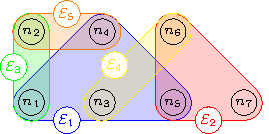
\includegraphics[width=\linewidth]{figures/hypergraph_diagram_1_standalone/figure.pdf}
        \caption{Graphical representation of $\s H$.}
        \label{fig:hypergraph_diagram_example}
    \end{subfigure}
    \begin{subfigure}{0.8\linewidth}
        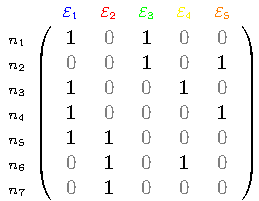
\includegraphics[width=0.8\linewidth]{figures/hypergraph_matrix_1_standalone/figure.pdf}
        \caption{Matrix representation of $\s H$.}
        \label{fig:hypergraph_matrix_example}
    \end{subfigure}
    \caption{Two different representations of a hypergraph $\s H$ which has $5$ hyperedges and $7$ nodes.}
    \end{figure}

    \begin{definition}
        A \term{weighted hypergraph} is an ordered pair $\s W = \br{\s H, \w}$ consisting of a hypergraph $\s H$ and corresponding \textit{weighting} $\w \in \Z_{\geqslant 1}^{\s E}$ over the edges of $\s H$.
    \end{definition}

    \begin{definition}
        A \term{transversal} of a weighted hypergraph $\s W = \br{\s H, \w}$ is a positive-integer solution $t \in \Z_{\geqslant0}^{\s N}$ of the following system of linear inequalities:
        \[ t \cdot \s H \succcurlyeq \w \iff \forall \s E \in \s H, \, \sum_{n \in \s E}t_{n} \defined t \cdot \s E \geqslant \w_{\s E} \eq \label{eq:primary_hypergraph_inequality_equation} \]
        The space of all transversals will be denoted $\mathscr{T}_{\succcurlyeq}\br{\s W}$.
    \end{definition}

    \begin{definition}
        A transversal $t \in \mathscr{T}_{\succcurlyeq}\br{\s W}$ is \term{minimal} if
        \[ \nexists t' \in \mathscr{T}_{\succcurlyeq}\br{\s W}, \, t'\neq t \text{ and } t' \preccurlyeq t. \]
        The space of all minimal transversals will be denoted $\mathscr{T}^{*}_{\succcurlyeq}\br{\s W}$.
    \end{definition}

    In the special case where $\w = \mathbf{1}$\footnote{Here $\mathbf{1}$ denotes the vector containing all ones.}, one recovers the notion of a transversal $t \in \bc{0,1}^{\nodes}$ of an \textit{unweighted} hypergraph; $t \cdot \s H \succeq \mathbf{1}$ if and only if the support of $t$ intersects every hyperedge of $\s H$, i.e. $\forall \s E, \, t \cdot \s E \neq 0$.

    The purpose of \cref{sec:algorithm_section} is to provide an algorithm which, when given a weighted hypergraph $\s W$, outputs all minimal transversals $\mathscr{T}^{*}_{\succcurlyeq}\br{\s W}$. Procedurally, the algorithm operates inductively over an arbitrary ordering of the hyperedges in $\s W$. It begins by minimally solving the first inequality $t \cdot \s E_1 \geqslant \w_{\s E_1}$ of \cref{eq:primary_hypergraph_inequality_equation} and then subsequently solving the the $(k+1)$-th inequality $t \cdot \s E_{k+1} \geqslant \w_{\s E_{k+1}}$ given a minimal solution for first $k$ inequalities. By construction, these \textit{partial} solutions are transversals of a partial weighted hypergraph.
    \begin{definition}
        The \term{partial weighted hypergraph} $\s W_{k}$ of $\s W = \br{\s H, \w}$ is a weighted hypergraph consisting of the first $k$ hyperedges of $\s H$ and corresponding weights from $\w$.
        \begin{align*}
            \s W &= \br{\s H, \w} = \br{\bc{\s E_1, \ldots, \s E_q}, \bc{\w_{\s E_1}, \ldots, \w_{\s E_q}}} \\
            \s W_{k} &= \br{\bc{\s E_1, \ldots, \s E_k}, \bc{\w_{\s E_1}, \ldots, \w_{\s E_k}}} \qquad 1 \leq k \leq q
        \end{align*}
    \end{definition}

    In the special case of $\w = \mathbf{1}_{\edges}$, it is customary to identify a class of hypergraphs known as \textit{simple} or \textit{Sperner} hypergraphs wherein $\forall i, j : \edges_i \subseteq \edges_j \Rightarrow j = i$ \cite{Berge_1984}. Non-simple hypergraphs possess a redundancy: whenever $\edges_i \subset \edges_j$, any $t \subseteq \nodes$ which satisfies $t \cap \edges_i \neq 0$ automatically satisfies $t \cap \edges_j \neq 0$ and hence any such $\edges_j$ can be ignored by any transversal generation algorithm. Analogous redundancies are absent from the $\w$-transversal generation problem because $\w \in \Z_{\geq 1}^{\edges}$ is arbitrary.

    \subsection{Generalized Nodes}

    In the original algorithm of \citet{Kavvadias_2005}, the concept of a \textit{generalized node} was introduced in order to improve the total running time and reduce memory requirements. The algorithm presented in \cref{sec:algorithm_section} also utilizes these generalized nodes and benefits significantly by reducing the number of intermediate partial transversals.

    Let $\s X_{k}$ be the generalized nodes of $\s H_{k}$. The generalized nodes $\s X_{k+1}$ of $\s H_{k+1} = \s H_{k} \cup \bc{\edges_{k+1}}$ can be computed using only $\s X_{k}$ and $\edges_{k+1}$. The following procedure accomplishes this as well as classifies each
    \begin{itemize}
        \item[($\al$)] If $X \cap \edges_{k+1} = \emptyset$, then $X \in \s X^{\al}_{k+1}$.
        \item[($\be$)] If $X \subseteq \edges_{k+1}$, then $X \in \s X^{\be}_{k+1}$.
        \item[($\ga$)] If $X \cap \edges_{k+1} \neq \emptyset$ and $X \not \subseteq \edges_{k+1}$, then
        \begin{itemize}
            \item[($\ga_1$)] $X \setminus \br{X \cap \edges_{k+1}} \in \s X^{\ga_1}_{k+1}$,
            \item[($\ga_2$)] $X \cap \edges_{k+1} \in \s X^{\ga_2}_{k+1}$.
        \end{itemize}
    \end{itemize}
    As a special case, if $\edges_{k+1}$ introduces any new nodes not captured by $\s X_{k}$, these nodes form a unique type $\de$ in $\s X_{k+1}$.
    \begin{itemize}
        \item[($\de$)] If $\de X \defined \edges_{k+1} \cap \br{\bigcup_{X \in \s X_{k}} X}$, then $\de X \in \s X_{k+1}^{\de}$.
    \end{itemize}

    \begin{figure}
        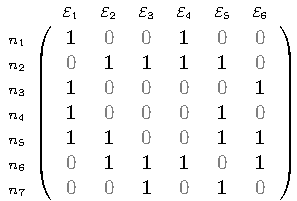
\includegraphics[width=\linewidth]{figures/hypergraph_matrix_2_standalone/figure.pdf}
        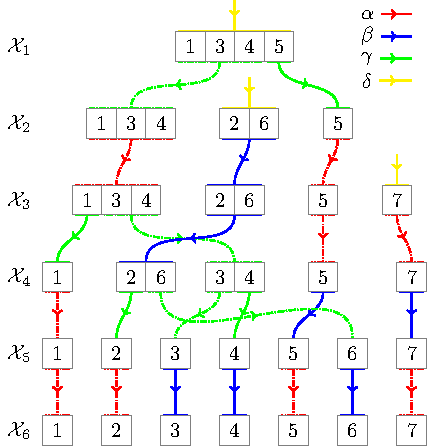
\includegraphics[width=\linewidth]{figures/generalized_node_tree_2/figure.pdf}
        \caption{The Generalized Node Tree of a hypergraph $\s H$ which has $6$ hyperedges and $7$ nodes.}
    \end{figure}


    \subsection{An Algorithm}
    \label{sec:algorithm_section}
    \begin{algorithm}[htp]
        \SetKwFunction{WKS}{WKS}
        \SetKwInOut{Input}{Input}
        \SetKwInOut{Output}{Output}
        \SetKwProg{Procedure}{Procedure}{:}{}
        \label[algorithm]{alg:WKS}
        \Procedure{\WKS{$\s G$, $U$, $\ep$}}{}
        \Input{An instruction set $\s G$, a unitary $U$, and accuracy $\ep > 0$}
        \Output{$S \in \ba{\s G}$ such that $d\br{S_{\times}, U} < \ep$}
        Choose $\eta \geq \s O \br{\f{d^2 - 1}{\log \abs{\s G}} \log \br{1 / \ep}}$ \\
        $T \leftarrow \bigcup_{\ell = 0}^{\eta} \s G^{\ell}$ \\
        \For{$S \in T$}{
            $S_{\times} \leftarrow \prod_{g \in S} g$ \\
            \If{$d\br{S_{\times}, U} < \ep$}{
                return S
            }
        }
        \caption{Generation of Minimal Solutions}
    \end{algorithm}
    \begin{algorithm}[htp]
        \caption{Canonical Minimalization Procedure}
        \SetKwFunction{CanonicalMinimal}{CanonicalMinimal}
        \SetKwInOut{Input}{Input}
        \SetKwInOut{Output}{Output}
        \SetKwProg{Procedure}{Procedure}{:}{}
        \label[algorithm]{alg:canonical_minimal}
        \Procedure{\CanonicalMinimal{$\s W$, $t$}}{}
        \Input{A weighted hypergraph $\s W = \br{\s H, \w}$ and a transversal $t \in \mathscr{T}_{\succcurlyeq}\br{\s W}$.}
        \Output{A minimal transversal $\Ga_{\s W}\br{t} \in \mathscr{T}^{*}_{\succcurlyeq}\br{\s W}$ such that $\Ga_{\s W}\br{t} \preccurlyeq t$.}
        \For{$n \in \si\br{t}$}{
            \If{$\br{t - \de_{n}} \in \mathscr{T}_{\succcurlyeq}\br{\s W}$}{
                \Return \CanonicalMinimal{$\s W$, $t-\de_{n}$}
            }
        }
        \Return $t$
    \end{algorithm}
    \begin{algorithm}[htp]
        \caption{Solving the $k$-th Inequality}
        \SetKwFunction{kSolve}{kSolve}
        \SetKwInOut{Input}{Input}
        \SetKwInOut{Output}{Output}
        \SetKwProg{Procedure}{Procedure}{:}{}
        \label[algorithm]{alg:kSolve}
        \Procedure{\kSolve{$t$, $\s W_{k-1}^{g}$, $\s X_{k}$}}{}
        \Input{A minimal transversal $t \in \mathscr{T}^{*}_{\succcurlyeq}\br{\s W_{k-1}^{g}}$, the associated generalized partial hypergraph $\s W_{k-1}^{g}$, and generalized nodes $\s X_{k}$ for $\s W_{k}^{g}$.}
        \Output{The set $\Ga^{-1}_{t}\br{\s W^{g}_{k-1}} \cap \mathscr{T}^{*}_{\succcurlyeq}\br{\s W_{k}^{g}}$ of minimal transversals of $\s W_{k}^{g}$ which are canonically minimal to $t$.}
        \For{$n \in \si\br{t}$}{
            \If{$\br{t - \de_{n}} \in \mathscr{T}_{\succcurlyeq}\br{\s W}$}{
                \Return \CanonicalMinimal{$\s W$, $t-\de_{n}$}
            }
        }
        \Return $t$
    \end{algorithm}

    \begin{definition}
        Given a set of generalized nodes $\s X$ for $\s N$, define the \term{unpacking operation} $\mathrm{U}_{\!\s X}$ which takes any vector $t \in \Z_{\geq 0}^{\s X}$ to a family of vectors $\mathrm{U}_{\!\s X}\br{t} \subset \Z_{\geq 0}^{\s N}$:
        \[ \mathrm{U}_{\!\s X}\br{t} \defined \bcm{t' \in \Z_{\geq 0}^{\s N}}{\forall X \in \s X, {\sum}_{n \in X} t'_{n} = t_{X}} \]
    \end{definition}
    \[ \abs{\mathrm{U}_{\!\s X}\br{t}} = \prod_{X \in \s X} \binom{t_{X} + \abs{X} - 1}{t_{X}} \]
    % \[ \mathbf{E}\br{\s H} = \bc{\s E_1, \ldots, \s E_q} \]
    % \[ \mathbf{N}\br{\s H} = \bc{n_1, \ldots, n_p} \]
    % \[ \mathbf{W}\br{\s H} = \bc{\w_1, \ldots, \w_q} \]
    % \[ \mathbf{W}\br{\s H_k} = \bc{\w_1, \ldots, \w_k} \]
    % \[ \mathbf{E}\br{\s H_k} = \bc{\s E_1, \ldots, \s E_k} \]
    % \[ \mathbf{N}\br{\s H_k} = \bc{n_1, \ldots, n_k} \]

    \[ \widetilde {\s T}_{\succeq \w_{k]}}\br{\s H_{k]}} = \mathrm{U}_{\!\s X_{k}}\br{\widetilde {\s T}_{\succeq \w_{k]}}^{\s X_{k}}\br{\s H_{k]}}} \]
    \[ \s X_{k} = \s X_{k}^{\al} \sqcup \s X_{k}^{\be} \sqcup \s X_{k}^{\ga_1} \sqcup \s X_{k}^{\ga_2} \sqcup \s X_{k}^{\de} \]
    \[ \s X_{k} \defined \s X_{k}^{\al,\be,\ga_1,\ga_2,\de} \]
    \begin{definition}
        \[ \s T\br{\s H, \w} \defined \bc{t \in \Z_{\geq 0}^{\nodes} \mid t \cdot \s H \succeq \w} \]
        \[ \widetilde {\s T}\br{\s H, \w} \defined \bc{t \in \s T\br{\s H, \w} \mid \nexists t' \in \s T\br{\s H, \w}, t' \neq t, t' \preceq t} \]
        \[ \s T_{k}\br{\s H, \w} \defined \bc{t \in \Z_{\geq 0}^{\nodes} \mid t \cdot \edges_i \geq \w_i, 1 \leq i \leq k} \]
        \[ \s T_{k}\br{\s H, \w} \defined \bc{t \in \Z_{\geq 0}^{\nodes} \mid t \cdot \s H \succeq_{k} \w} \]
        \[ \s T_{k}^{\s X}\br{\s H_{k]}, \w_{k]}} \defined \bc{t \in \Z_{\geq 0}^{\s X} \mid t \cdot \s H \succeq_{k} \w} \]
        \[ \s T\br{\s H^{g}_{k]}, \w_{k]}} \defined \bc{t \in \Z_{\geq 0}^{\nodes\br{\s H_{k]}^{g}}} \mid t \cdot \s H^{g}_{k]} \succeq \w_{k]}} \]
        Shorthand,
        \[ \s X_k \defined \nodes\br{\s H_{k]}^{g}} \]

        Begin with $\s T\br{\s H^{g}_{1]}, \w_{1]}} = \bc{t}$ which corresponds to a single generalized transversal $t \in \Z_{\geq 0}^{\s X_1}$. Since $\s X_k$ only contains one generalized node $\s X_1 = \bc{\edges_1}$, the initial generalized transversal has $t_{\s X_1} = \w_1$ ,
        \[  \]

        \[ \s T_{k}^{\s X}\br{, \w} \defined \bc{t \in \Z_{\geq 0}^{\s X} \mid t \cdot \s H \succeq_{k} \w} \]
        \[ \s T_{q}\br{\s H, \w} = \s T\br{\s H, \w} \]
        \[ \s T_{1}\br{\s H, \w} = \bc{t \in \Z_{\geq 0}^{\nodes} \mid t \cdot \edges_1 \geq \w_1} \]
        \[ \s T_{1}\br{\s H, \w} = \bc{t \in \Z_{\geq 0}^{\nodes} \mid t \cdot \edges_1 \geq \w_1} \]
        \[ \s T\br{\s H, \w} \defined \bc{t \in \Z_{\geq 0}^{\nodes} \mid t \cdot \edges_i \leq \w_i, 1 \leq i \leq q} \]
    \end{definition}

    Given the minimal solutions $\widetilde {\s T}\br{\s H_{k]}, \w_{k]}}$, how does one find the minimal solutions $\widetilde {\s T}\br{\s H_{k+1]}, \w_{k+1]}}$? Given a particular partial solution $t \in \widetilde {\s T}\br{\s H_{k]}, \w_{k]}}$


    \begin{definition}
        Given $t \in \widetilde {\s T}_{\succeq \w_{k]}}^{\s X_{k}}\br{\s H_{k]}}$, the \term{offspring} $\s O\br{t}$ of $t$ are all minimal $\w_{k]}$-transversals of $\s H_{k]}$ in terms of the generalized nodes $\s X_{k+1}$. $\s O\br{t}$ is the set of all $t' \in \Z_{\geq 0}^{\s X_{k+1}}$
        \begin{itemize}
            \item $\forall X \in \s X_{k+1}^{\al} \cup \s X_{k+1}^{\be}, t'_{X} = t_{X}$ and
            \item $\forall X_1 \in \s X_{k+1}^{\ga_1}, X_2 \in \s X_{k+1}^{\ga_2}$ such that $X_1 \cup X_2 \in \s X_{k}$
        \end{itemize}
    \end{definition}
    \[ \s E_{k+1} = \s X_{k+1}^{\be} \sqcup \s X_{k+1}^{\ga_2} \sqcup \s X_{k+1}^{\de} \]
    Given transversal $t$, each offspring $t' \in \s O\br{t}$ already covers edge $\s E_{k+1}$ an amount $\eta$.
    \[ \eta \defined t' \cdot \s E_{k+1} = \sum_{X \in \s X_{k+1}^{\be} \sqcup \s X_{k+1}^{\ga_2}} t_X \]
    If $\eta < \w_{k+1}$ then the offspring $t'$ needs to be supplemented by $s \in \Z_{\geq 0}^{\s X_{k+1}}$ such that $s$ covers the remaining weight for edge $\s E_{k+1}$. Explicitly, $s$ needs to be constructed such that,
    \[ s \cdot \s E_{k+1} = \sum_{X \in \s X_{k+1}^{\be, \ga_2, \de}} s_{X} = \w_{k+1} - \eta  \]
    \[ \s S\br{t'} \defined  t_X \]


    \section{Conclusions}

    \subsection{Unsolved}
    Consider $\ga_{1}, \ga_{2}$ and $\ga_{1} + \ga_{2}$.
    \[ I\br{\ga_a} = \bc{\br{\ga_{a} + \ti \ga_{a}} \cdot \prob{\mscenariowrap} \geq 0 \mid \ti \ga_{a} \in \transversals{\w\br{\ga_a}}{\s H\br{\ga_a}}} \quad a = 1,2 \]
    % \[ I\br{\ga_1 + \ga_2} = \bc{\br{\ga_{1} + \ga_{2} + \ti \ga_{12}} \cdot \prob{\mscenariowrap} \geq 0 \mid \ti \ga_{12} \in \transversals{\w\br{\ga_1}+\w\br{\ga_2}}{\s H\br{\ga_1 + \ga_2}}} \]

    \section*{Acknowledgments}

    \setlength{\bibsep}{3pt plus 3pt minus 2pt}
    \bibliographystyle{apsrev4-1}
    \nocite{apsrev41Control}
    \bibliography{references}

\end{document}
